\section{Styrhandske}
\begin{figure}[H]
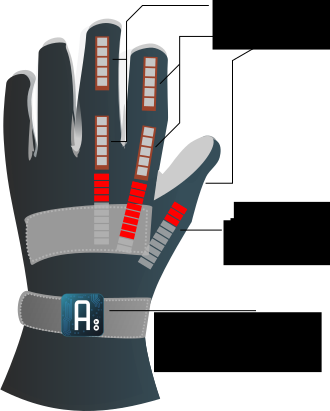
\includegraphics[height=0.5\textheight]{img/kontrollhandske}
\caption{Konceptskiss över styrhandsken.}
\label{kontrollhandske}
\end{figure}
%Detta är intro. Det ska inte vara några detaljer här, bara översiktligt!
% Konvention: styrhandske, inte reglerhandske eller kontrollhanske

För att intuitivt reglera robothanden används en tunn handske som användaren bär på sin hand, se \ref{styrhandskediod}. På handskens tumme, långfinger och pekfinger finns det två flexsensorer vardera, se figur \ref{kontrollhandske}, som följer användarens hand och ändrar resistans beroende på hur mycket de böjs. På handsken sitter det även tre ledramper som indikerar hur hårt man påverkar objektet. Det tänds fler ledlampor ju större trycket på trycksensorerna är. För att strömförsörja Arduinon, bluetoothmodulen och ledramperna används ett powerpack på 5 Volt, se referenslista i appendix \ref{chp:komponentlista}. Fullständigt kretsschema, se appendix \ref{schemahandske}.
 \begin{figure}[H]
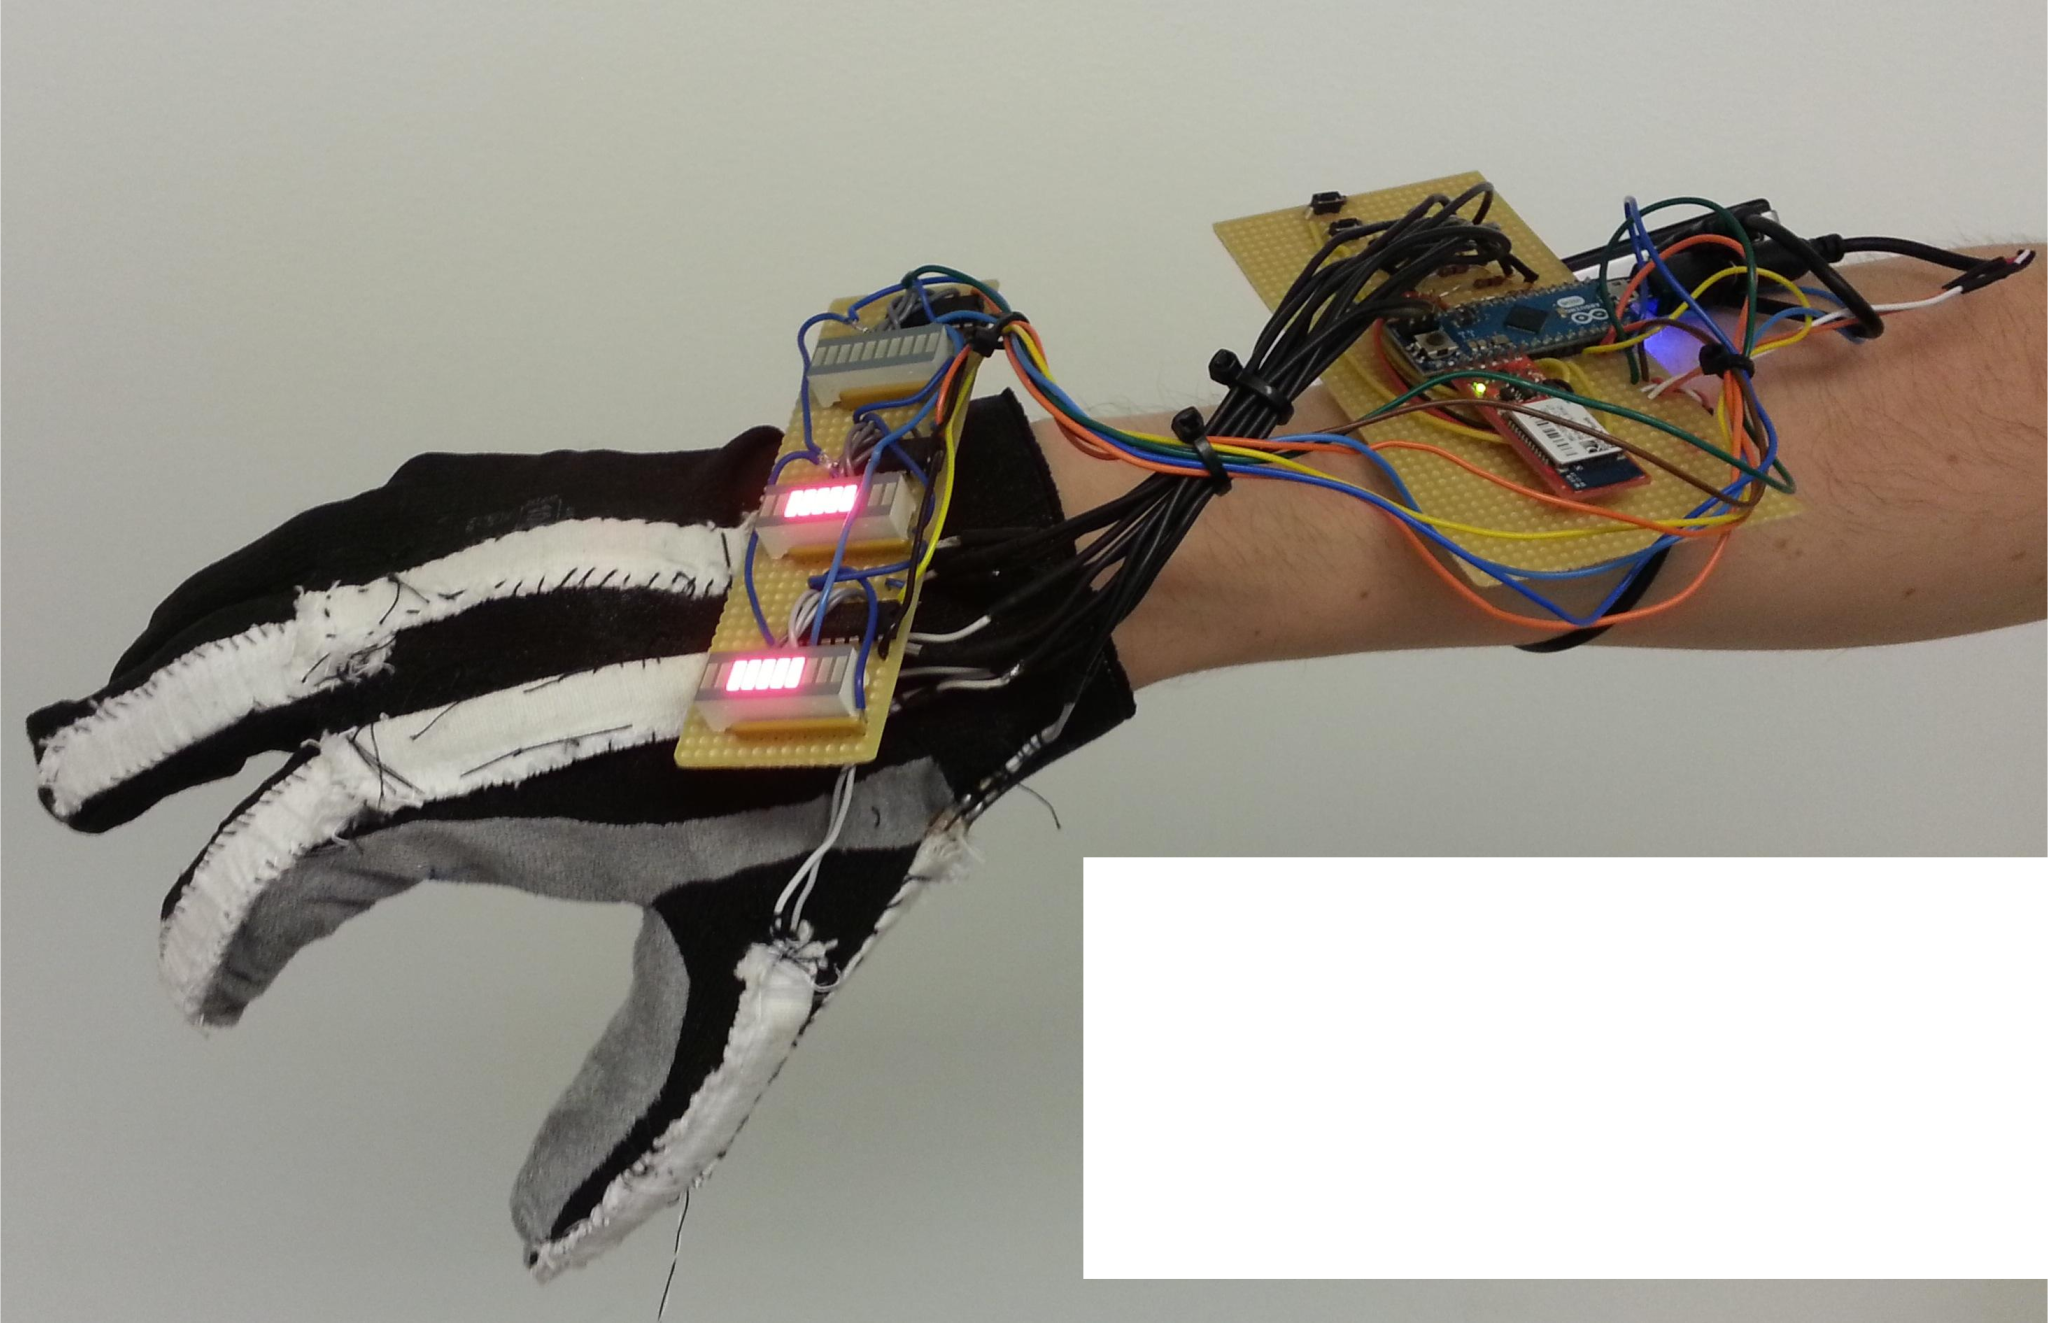
\includegraphics[height=0.4\textheight]{img/styrhandskediod}
\caption{Styrhandsken.}
\label{styrhandskediod}
\end{figure}







